\section*{Hard Tasks}

\subsection*{Landmark Relations}

As basic functionality, our tool allows to show certain objects attributed with
geographic position information, like buildings, parks, waters, districts in, and
photos taken of Berlin.
The user can click on each pair of those objects to get information about
relationships between those.
The tool takes the type of object into account and displays according
to feasibility the minimal distance between the objects, whether they lie
inside of each other, and how the objects intersect following the 9-cut model.

The photos we are using were fetched from the website Flickr tagged
as Brandenburg gate.
Therefore, we show them as points with a size proportional to
the distance of the place they were shot to this landmark.
Hovering over a photo displays the picture next to the mouse
as seen in \figref{brandenburg}.

\begin{figure}[b]
\centering
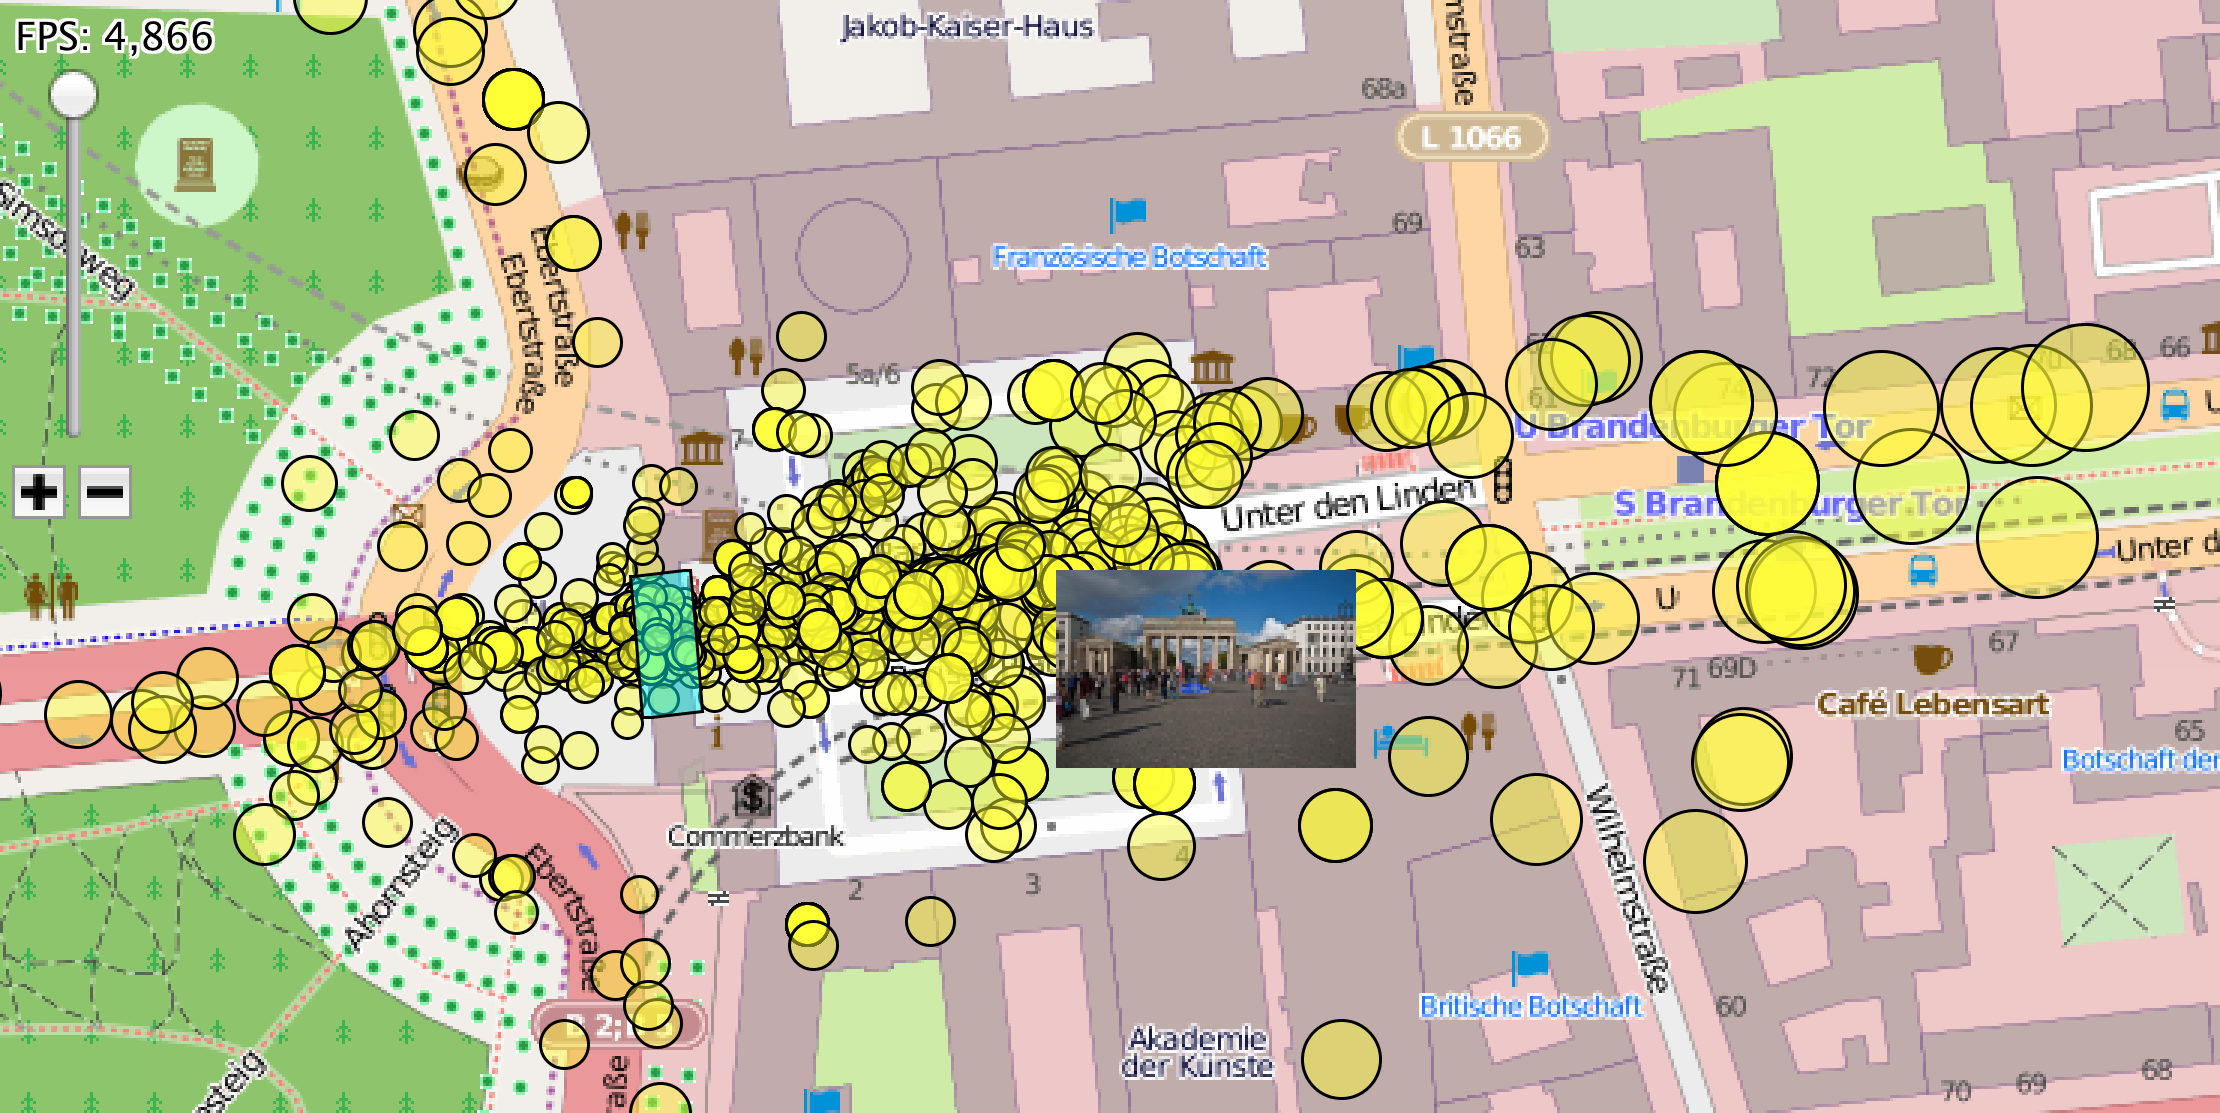
\includegraphics[width=0.9\linewidth]{imgs/brand}
\caption{Photos tagged as Brandenburg gate. The size of the dots
is proportional to the distance to the actual landmark.
A hovered photo shows the actual picture.}
\label{fig:brandenburg}
\end{figure}

\begin{figure}
        \centering
		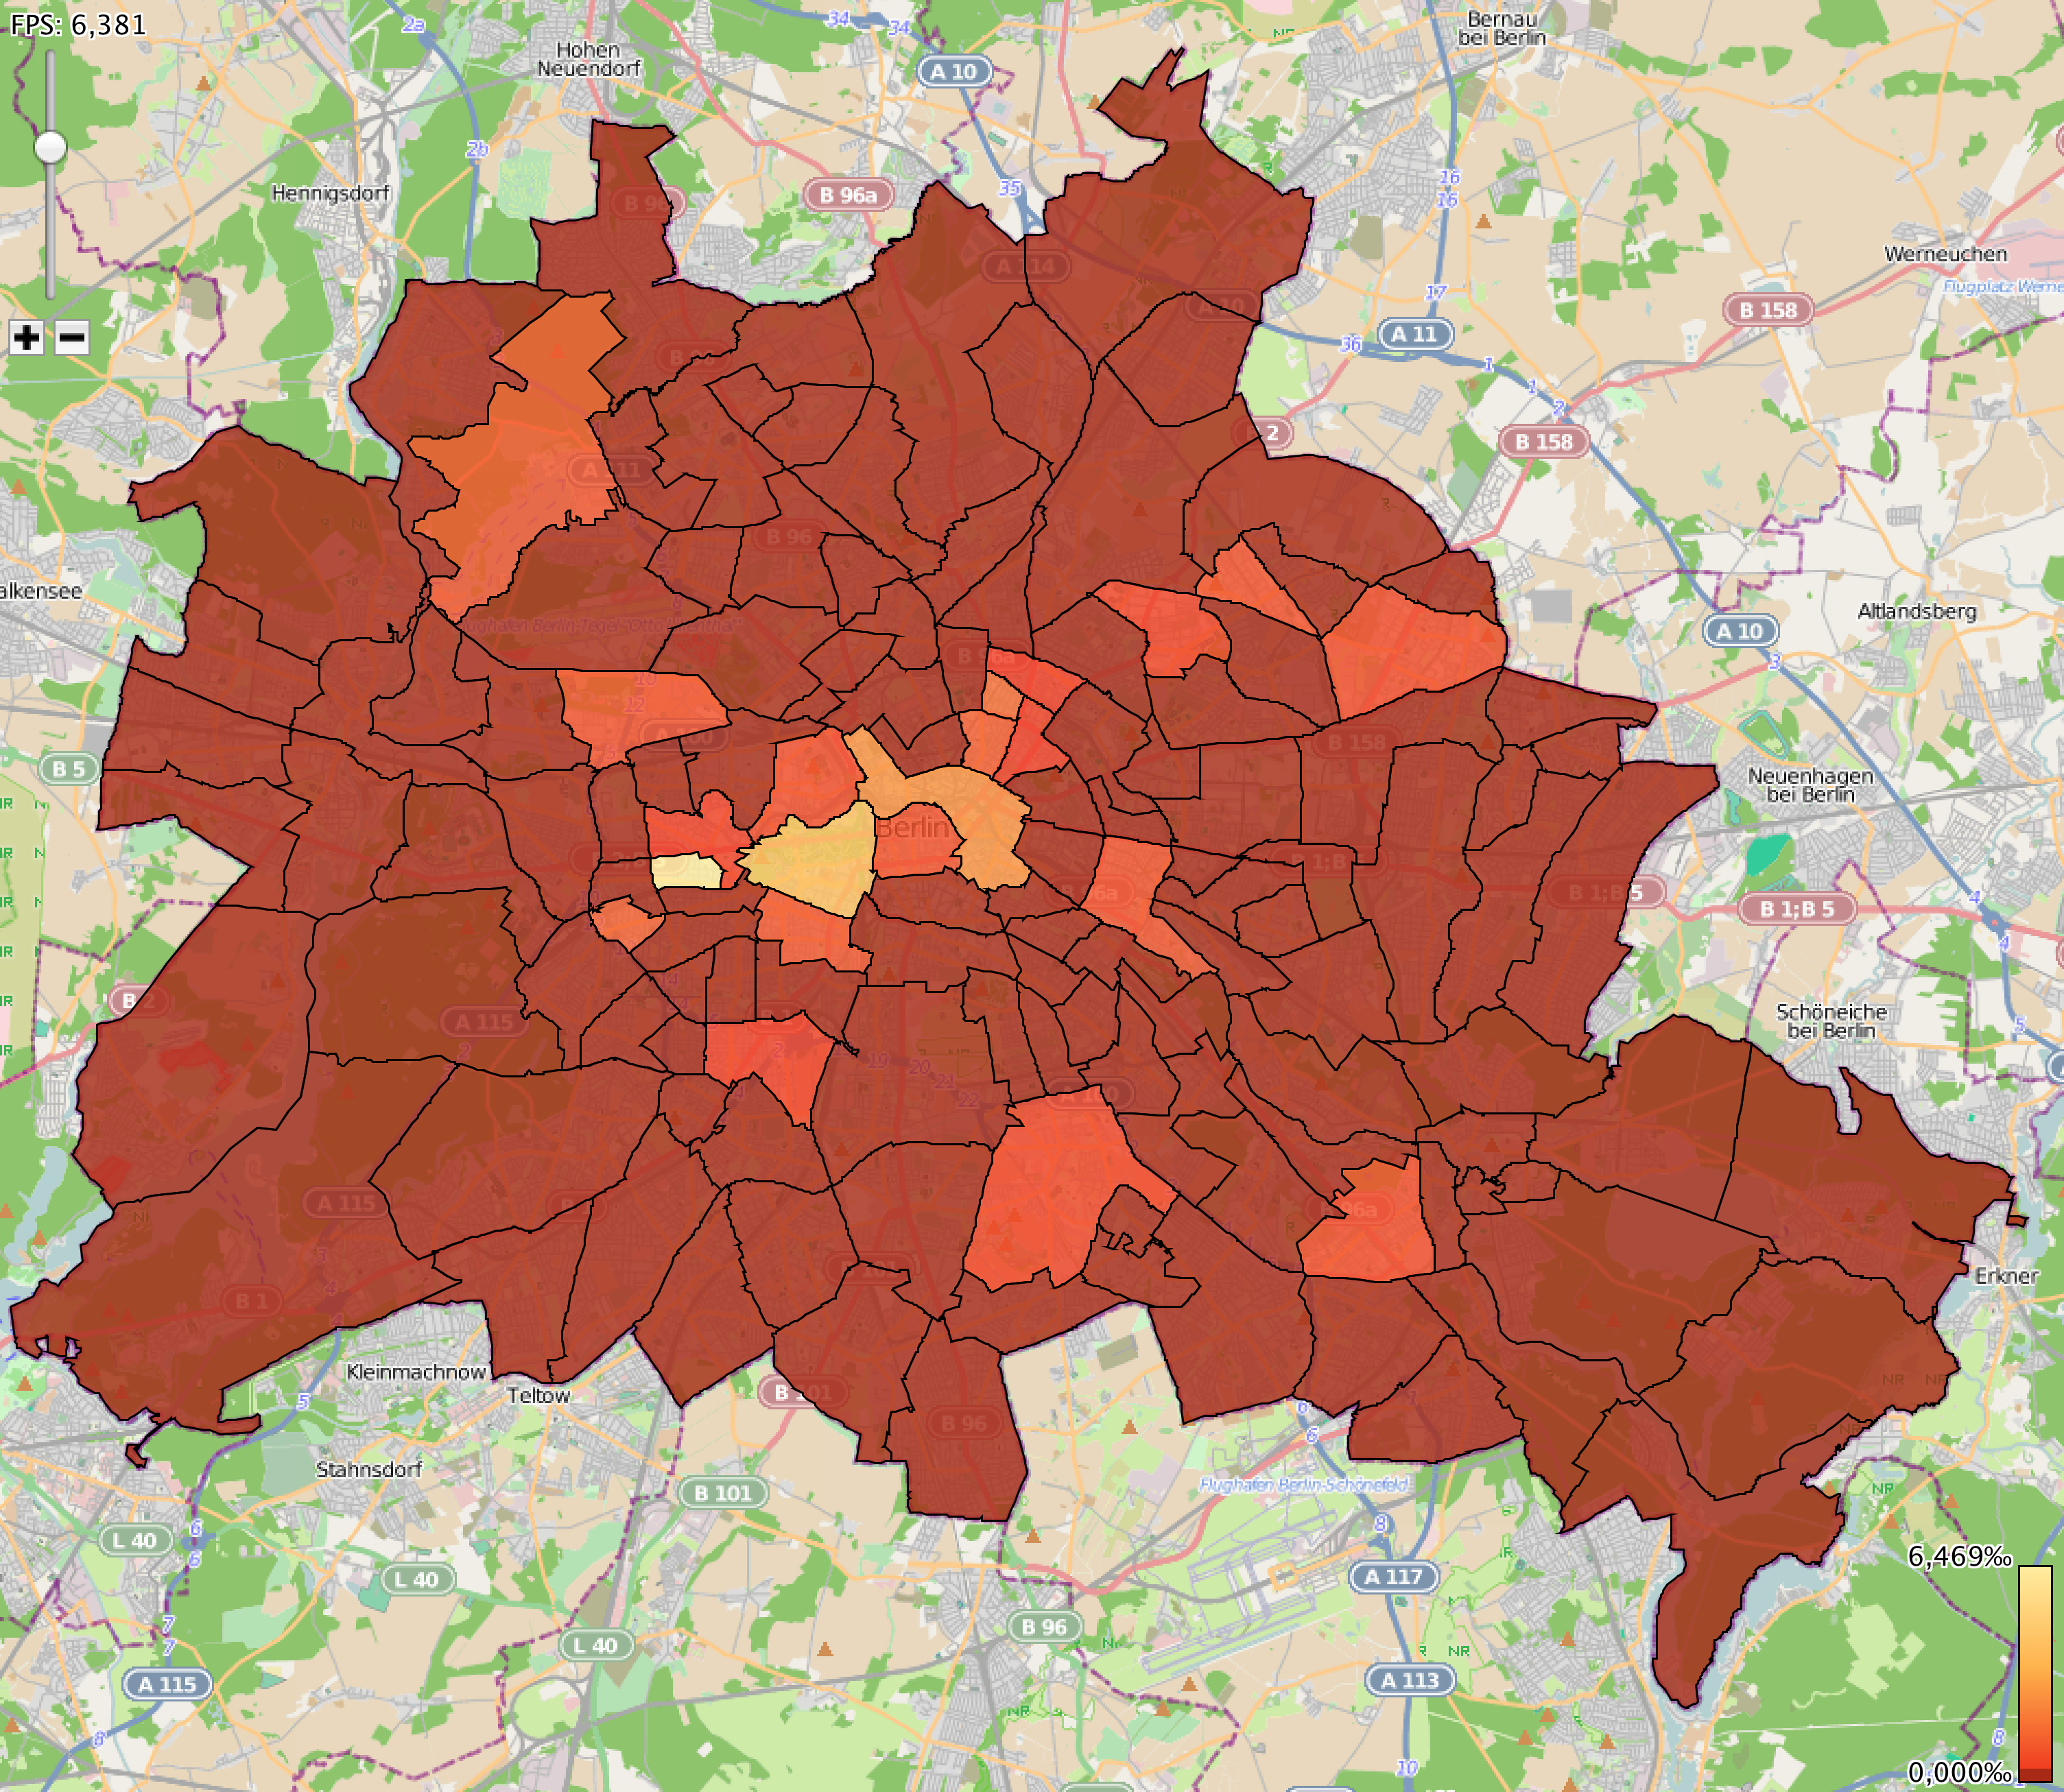
\includegraphics[width=0.8\linewidth]{imgs/commercial}
        \caption{A choropleth map showing the ratio of the area of commercial buildings
        per district to the area of the district.}
		\label{fig:commercial}
\end{figure}

\subsection*{Visual Analysis}

\todo{}

+

\todo{distance transformation explained}

\begin{figure*}[t]
		\centering
		\begin{subfigure}[b]{0.3\textwidth}
                \centering
                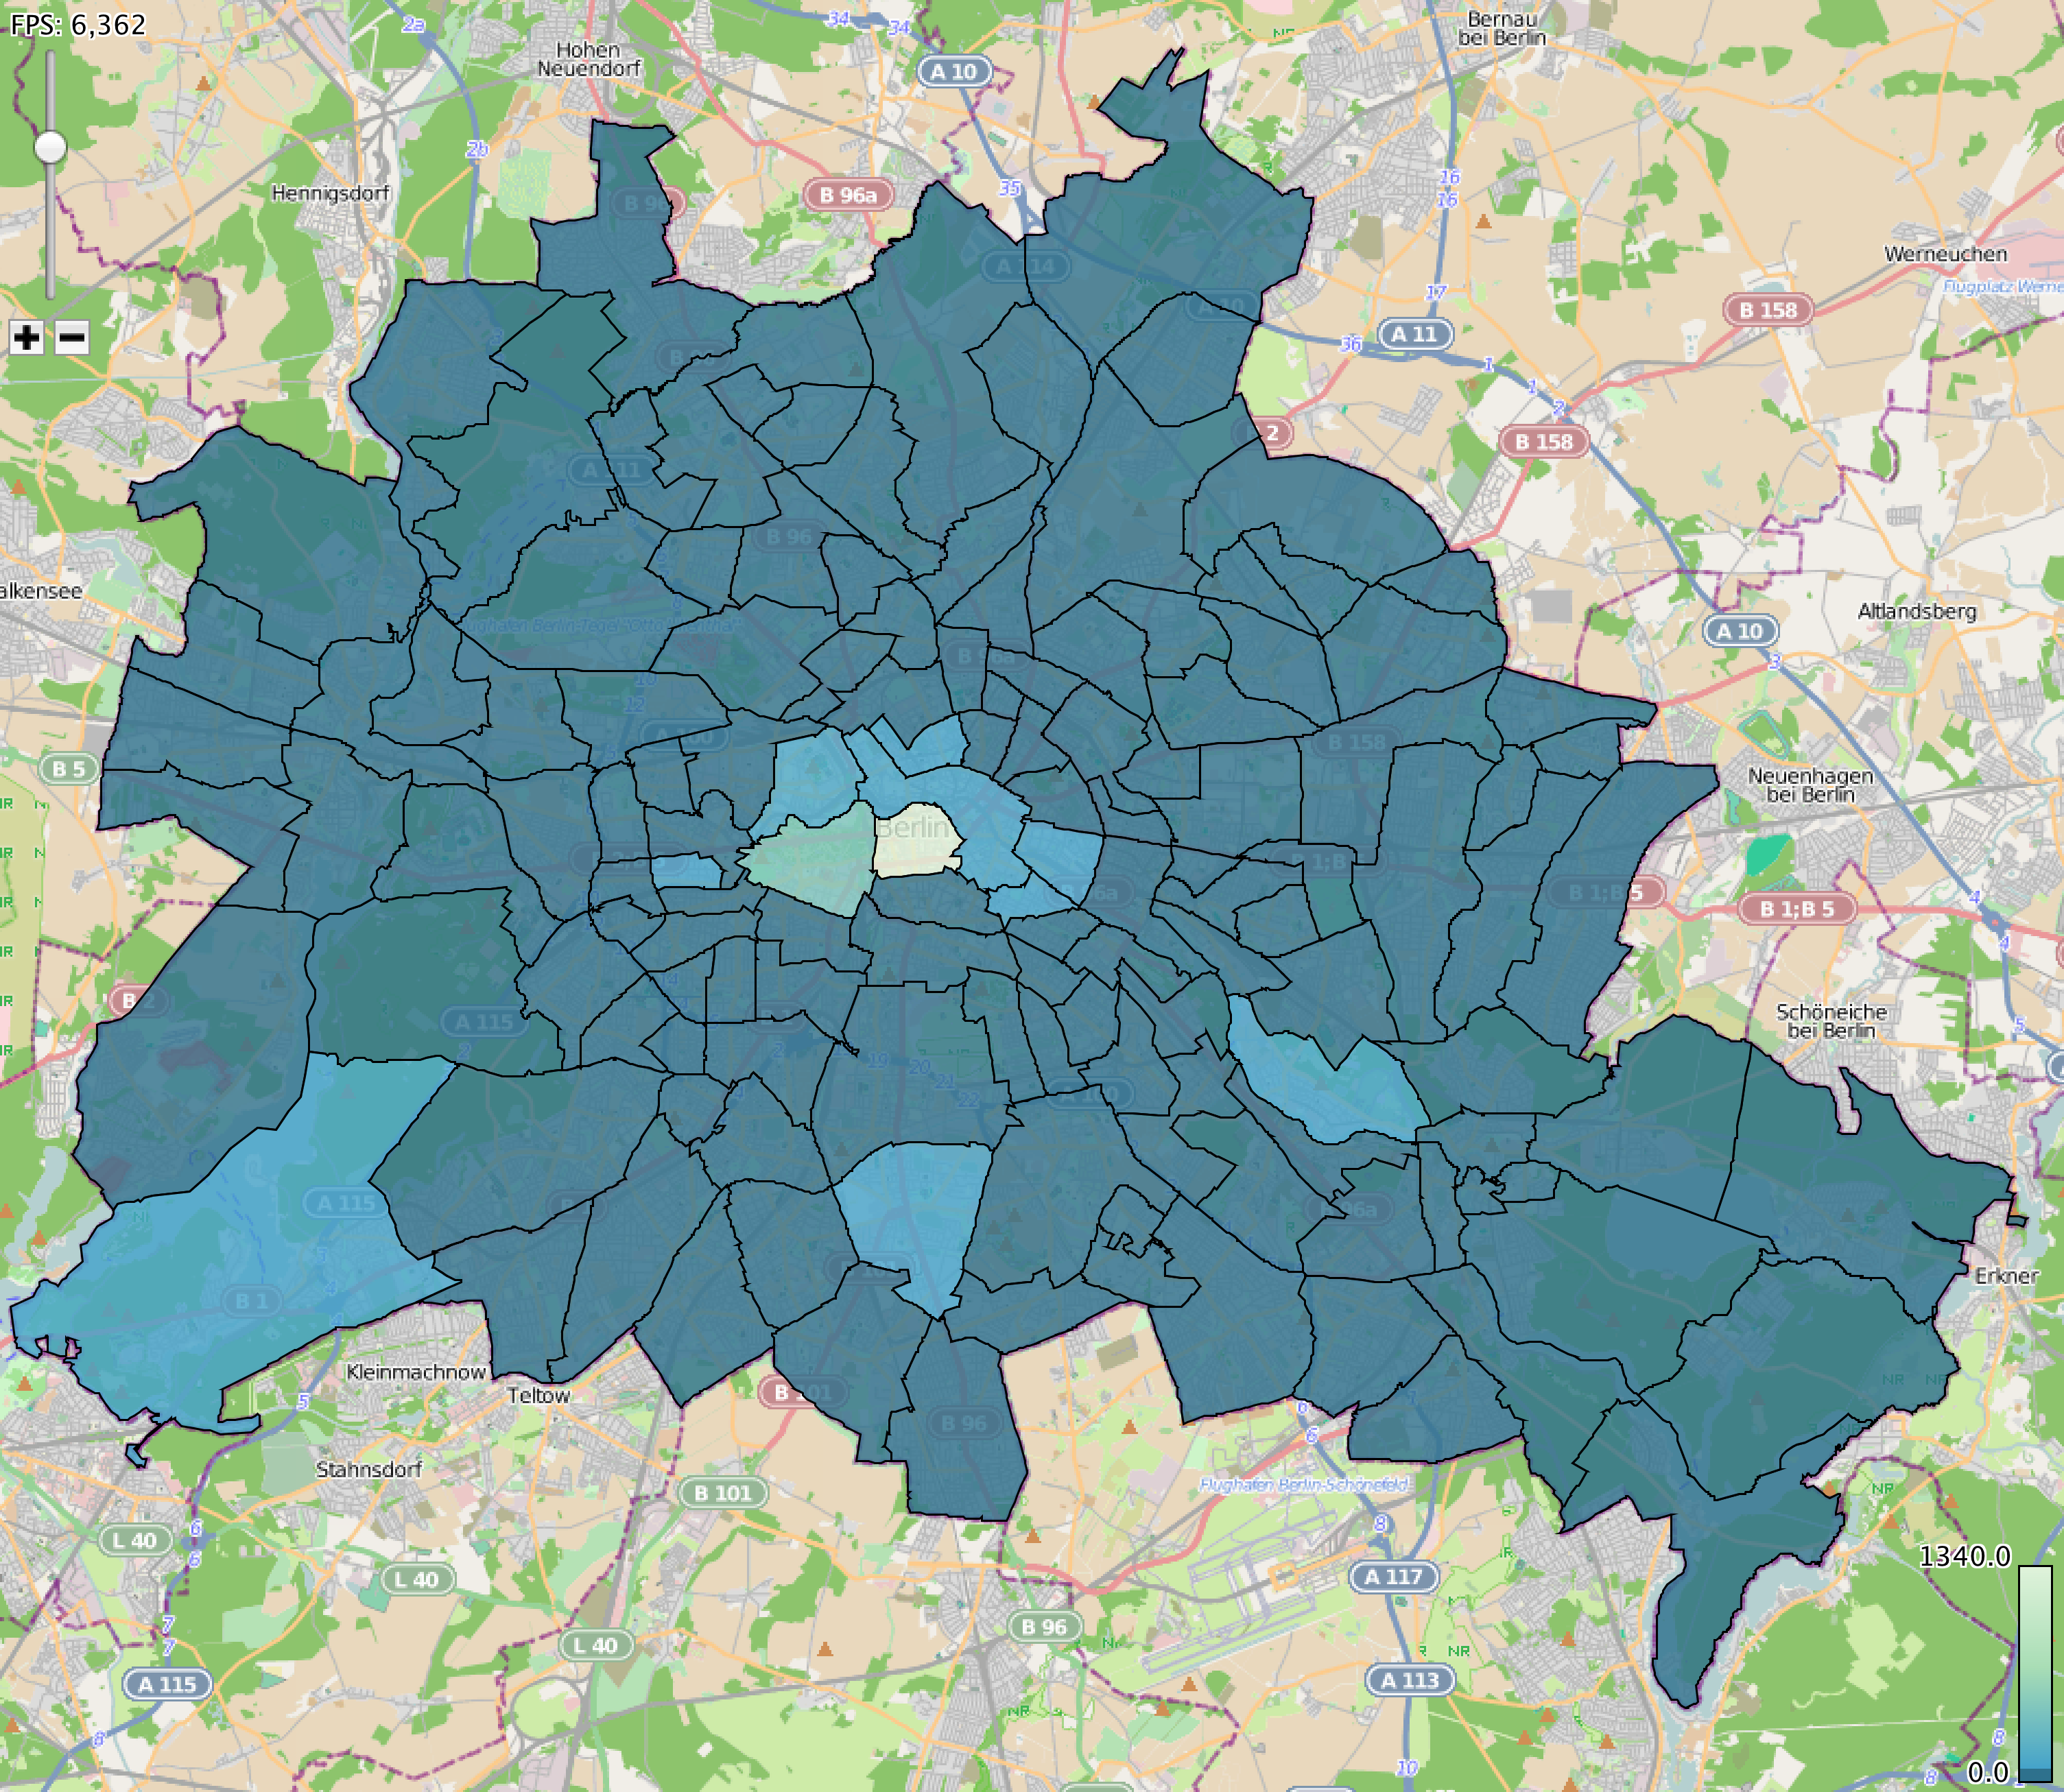
\includegraphics[width=\textwidth]{imgs/flickr}
                \caption{A choropleth map showing the relative amount of flickr photos tagged
                as Brandenburg gate in a given district.}
                \label{fig:flickr}
        \end{subfigure}
        \begin{subfigure}[b]{0.3\textwidth}
				\centering
				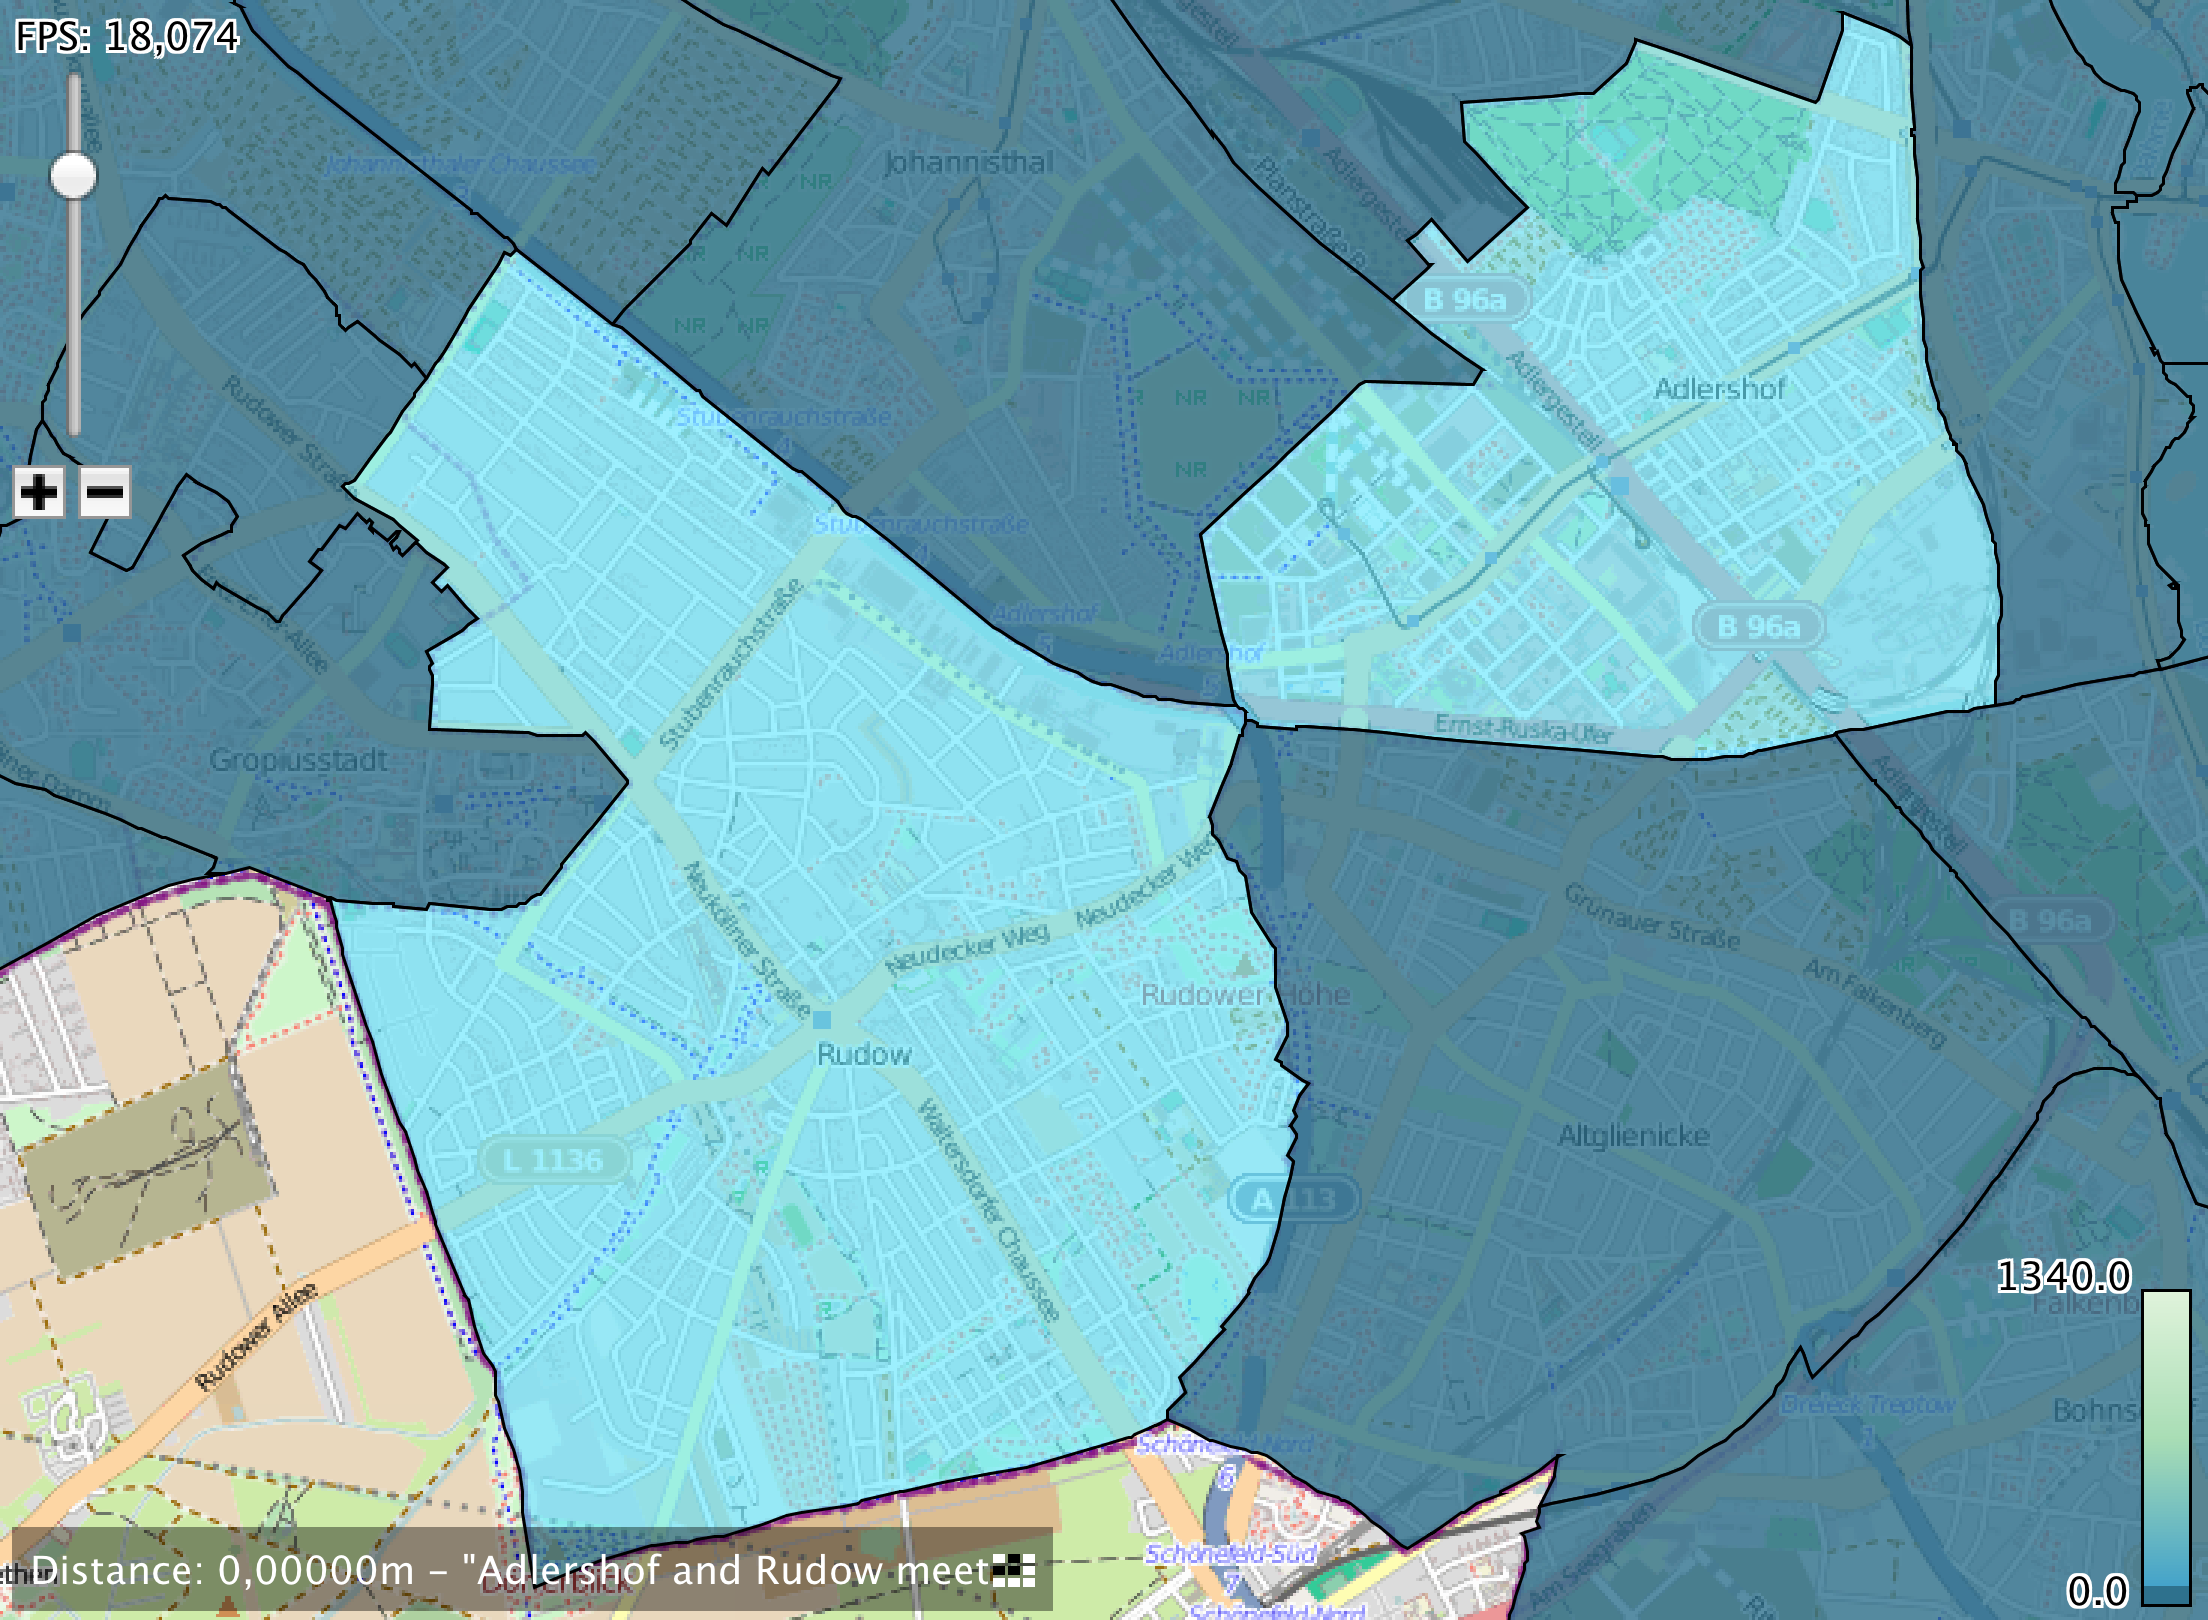
\includegraphics[width=\textwidth]{imgs/rel}
				\caption{A selection of two districts showing the message that
				they meet along with the corresponding 9-cut matrix.}
				\label{fig:rel}
		\end{subfigure}
        \begin{subfigure}[b]{0.3\textwidth}
                \centering
                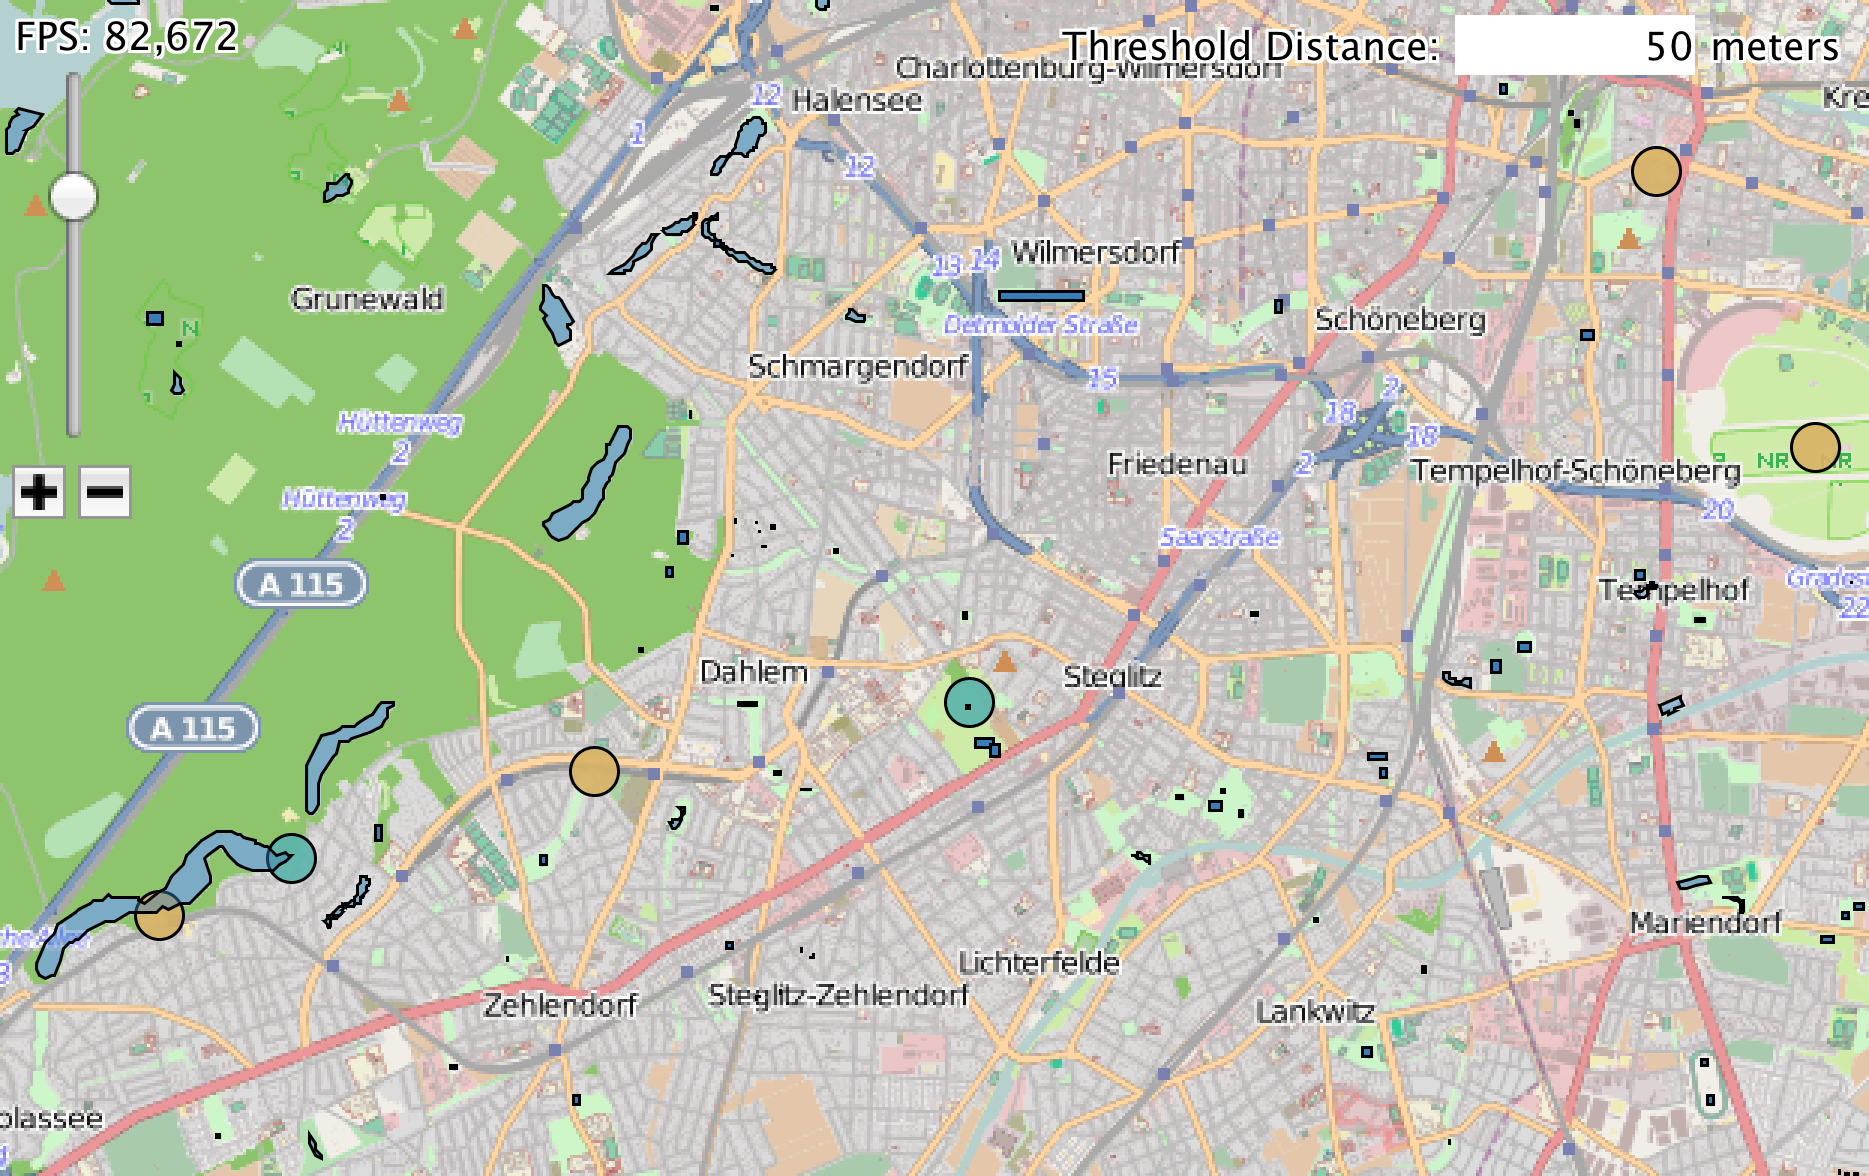
\includegraphics[width=\textwidth]{imgs/parks}
                \caption{\todo{}}
                \label{fig:parks}
        \end{subfigure}
        \caption{\todo{}}
\end{figure*}
